\chapter{Validaci\'on y Resultados}
\label{chap:resultados}

%\endinput

\section{Introducci\'on}
En este cap\'itulo se presentan los distintos escenarios que fueron planteados para la validaci\'on de los procesos.\\

Dado que para la metodolog\'ia de estimaci\'on de errores que proponemos, utilizamos datos reales de una misi\'on operativa argentina, hubiera sido
deseable contar con datos de alertas de colisiones reales propios de esa misi\'on, ya que esto hubiera permitido hacer una validaci\'on end-to-end de todo el prototipo. No obstante, por cuestiones de confidencialidad, no fue posible tener acceso a esa informaci\'on.
Frente a este panorama, se detalla a continuaci\'on la secuencia de etapas de validaci\'on que permiten evaluar, cada una de las instancias del procesamiento.\\

En primer lugar fue fundamental corroborar las propagaciones de los TLE realizadas con la librer\'ia de python {\it{sgp4-1}} \citep{sgp4python}, para ello utilizamos la versi\'on de prueba que ofrece el software STK: {\it{System Tool Kit}}, \citep{stk}.\\

Para la validaci\'on de los resultados de la implementaci\'on del m\'etodo de Osweiler en la generaci\'on de matrices de covarianza, se compararon los resultados de ARxCODE para dos de los escenarios que se publican en el trabajo.\\

El m\'etodo que se propone para la estimaci\'on de la propagaci\'on de errores, es el que m\'as dificultades present\'o para ser validado. Al basarse plenamente en los datos de la misi\'on cuyos resultados de colisi\'on de alerta no pudieron ser suministrados, fue analizado en comparaci\'on con resultados estad\'isticos globales, o sobre el estudio de encuentros de otras misiones.\\

Finalmente la implementaci\'on del c\'alculo de probabilidad de colisi\'on fue evaluada a partir de registros p\'ublicos de encuentros anteriores recopilados de internet en formato de correos electr\'onicos o CDM; y tomando datos de estudios publicados en el libro de Klinkrad \citep{Klinkrad} y en el trabajo de Xu y Xiong \citep{xu2014method}\\

\section{Implementaci\'on del modelo SGP4 en Python}

Para la propagaci\'on de las posiciones orbitales con el modelo SGP4 (Sec. \ref{subsec:sgp4model}) utilizamos la librer\'ia de python {\bf{sgp4-1}} \citep{sgp4python}.
Luego usamos el software STK para comparar nuestras propagaciones y asegurarnos la correcta utilizaci\'on y configuraci\'on de la librer\'ia sgp4-1.\\

Las Tablas \ref{tab:arcode}  y \ref{tab:stk} muestran las efem\'erides de la misi\'on operativa durante los primeros cuatro minutos del d\'ia 01/01/2013.
Ambas fueron generadas a partir del mismo TLE y presentan resultados que difieren en algunos metros para los peores casos. Resultado aceptable, teniendo en cuenta que las estimaciones groseras de errores para las propagaciones hechas con TLEs y SGP4 acarrean errores de kil\'ometros o decenas de kil\'ometros.\\

\underline{TLE.}
{\small
\begin{verbatim}
1 xxxxU xxxxx   13001.74853505  .00000428  00000-0  75550-4 0  9996
2 xxxxx 098.0122 011.5654 0001526 107.5603 009.0604 14.72289948 84036
\end{verbatim}}


\begin{table}[!h]
\caption{Resultados que genera ARxCODE utilizando la librer\'ia sgp4 de python para la propagaci\'on.}
\centering
\resizebox{17cm}{!}{
\begin{tabular}{lcccccc}
\hline
Epoca & x [km] & y [km] & z [km] & vx $[km/s]$ & vy $[km/s]$ & vz $[km/s]$\\
\hline
2013-01-01 00:00&-2372.76245& -1381.01830& 6465.57494& -6.95099& -0.93631& -2.74523\\
2013-01-01 00:01& -2784.64672& -1434.31269& 6287.6158& -6.77374& -0.83955& -3.18470\\
2013-01-01 00:02& -3185.05363& -1481.69530& 6083.67196& -6.56854& -0.73932& -3.61109\\
2013-01-01 00:03& -3572.3305& -1522.96975& 5854.58154& -6.336229& -0.63602& -4.02263\\
2013-01-01 00:04& -3944.8780& -1557.96472& 5601.28702& -6.077737& -0.53007& -4.417616\\
\hline
\label{tab:arcode}
\end{tabular}
}
\end{table}

\begin{table}[!h]
\caption{Resultados del Systems Tool Kit (STK) propagando el mismo TLE que ARxCODE.}
\centering
\resizebox{17cm}{!}{
\begin{tabular}{lcccccc}
\hline
\'Epoca & x [km] & y [km] & z [km] & vx [km/s] & vy [km/s] & vz [km/s]\\
\hline
2013-01-01 00:00&-2372.76302&-1381.02018&6465.57433&-6.95099&-0.93631&-2.74523\\
2013-01-01 00:01&-2784.64726&-1434.31473&6287.61518&-6.77374&-0.83955&-3.18470\\
2013-01-01 00:02&-3185.05413&-1481.69750&6083.67116&-6.56854&-0.73932&-3.61109\\
2013-01-01 00:03&-3572.33097&-1522.97210&5854.58064&-6.33622&-0.63602&-4.02263\\
2013-01-01 00:04&-3944.87849&-1557.96721&5601.28604&-6.07773&-0.53008&-4.41761\\
\hline
\label{tab:stk}
\end{tabular}
}
\end{table}


%\textcolor{red}{hacer las diferencias medias para todo un dia en python y publicarlas}

\section{Estudio de errores de TLE con datos hist\'oricos}

El trabajo de Osweiler publica los resultados de las matrices de covarianza generadas, para 6 misiones y 8 ventanas de tiempo.
Para la validaci\'on se tomaron dos escenarios muy diferentes en cuanto a la altura del sat\'elite: LAGEOS-1 a m\'as de $5000$ km y ICESAT a $600 $ km, (Tabla \ref{tab:satescenarios}).

\begin{table}[!h]
\caption[Sat\'elites de Estudio]{Resumen de las caracter\'isticas de los sat\'elites a analizar.}

      \begin{tabular}{cccccc}
      \hline
      Nombre & ID NORAD & Altura & Ecc. & Inclinaci\'on & B* \\
      \hline
      LAGEOS-1 & 8820 & $5850$ & $0.004$ & $109.8$ & $0.0001$ \\
      ICESAT & 27642 & $600$ & $0.0002 - 0.001$ & $94$ & var\'ia \\
      \hline
      \end{tabular}
    \label{tab:satescenarios}
\end{table}

Se presentan a continuaci\'on las tablas con los resultados comparativos, entre los valores publicados (Tablas \ref{tab:icesatOSW} y \ref{tab:lageosOSW}) y los valores obtenidos por ARxCODE (Tablas \ref{tab:icesatARX} y \ref{tab:lageosARX}) para una \'unica ventana temporal.\\

Puede apreciarse, que los errores son muy grandes para el ICESAT, de baja altura, que se ve m\'as perturbado por el efecto atmosf\'erico, que no es modelable con precisión; mientras que el LAGEOS-1 presenta errores muchos \'ordenes de magnitud menor.\\

\subsection*{Tablas comparativas ICESAT}

\begin{table}[!h]
\centering
\makebox[0pt][c]{\parbox{1.0\textwidth}{%
    \begin{minipage}[t]{0.48\hsize}
    \caption{Matriz de Covarianza. \citep{osweiler} \\ ICESAT del 1-Mar-03 al 16-Mar-03.}
     \resizebox{8cm}{!}{
    \begin{tabular}{cccc}
      \hline
    Vent 1 & $R_{v}$ (km) & $R_{n}$ (km) & $R_{c}$ (km)\\
    \hline
    $R_{v}$ &  2667.377375  &    27.248658   &   -8.22221222\\
    $R_{n}$ & 27.248658  &   0.34323269 & -0.12314379\\
    $R_{c}$ & -8.22221222 & -0.12314379 & 0.07316443\\
    \hline
    \end{tabular}}
      \label{tab:icesatOSW}
    \end{minipage}
    \begin{minipage}[t]{0.48\hsize}
    \caption{Matriz de Covarianza de ARxCODE. \\ ICESAT del 1-Mar-03 al 16-Mar-03.}
    \resizebox{8cm}{!}{
      \begin{tabular}{cccc}
	\hline
      Vent 1 & $R_{v}$ (km) & $R_{n}$ (km) & $R_{c}$ (km)\\
      \hline
      $R_{v}$ &  2667.37364259 &   27.2488814  &   -8.22232626\\
      $R_{n}$ & 27.2488814  &  0.3432413 &  -0.12314867\\
      $R_{c}$ & -8.22232626 & -0.12314867 &  0.073167\\
      \hline
      \end{tabular}}
        \label{tab:icesatARX}
    \end{minipage}
 %   \hfill
}}
\end{table}

\begin{table}[!h]
\caption{Diferencias de ARxCODE respecto a Osweiler \citep{osweiler}}

  \begin{tabular}{cccc}
  \hline
 Vent 1 & Dif.$R_{v}$ (km) & Dif.$R_{n}$ (km) & Dif.$R_{c}$ (km)\\
 \hline
 Dif. $R_{v}$ & -0.00373241 & 0.0002234 & -0.00011404 \\
 Dif. $R_{n}$ &  0.0002234 &  0.000008 & -0.000004\\
 Dif. $R_{c}$ & -0.00011404  & -0.000004 &  0.000002\\
 \hline
 \end{tabular}
 \label{tab:icesatcomp}
\end{table}


\subsection*{Tablas comparativas LAGEOS-1}

\begin{table}
\centering
\makebox[0pt][c]{\parbox{1.0\textwidth}{%
    \begin{minipage}[b]{0.48\hsize}
    \caption{Matriz de Covarianza. \citep{osweiler} \\ LAGEOS-1 del 1-Mar-03 al 16-Mar-03}
    \resizebox{8cm}{!}{
      \begin{tabular}{cccc}
	\hline
      Vent 1 & $R_{v}$ (km) & $R_{n}$ (km) & $R_{c}$ (km)\\
      \hline
      $R_{v}$ &  0.37863904 & -0.03440871 & 0.02772177 \\
      $R_{n}$ & -0.03440871 & 0.00401173 & -0.00272334 \\
      $R_{c}$ & 0.02772177 & -0.00272334 & 0.00843443\\
      \hline
      \end{tabular}}
        \label{tab:lageosOSW}
    \end{minipage}
    \hfill
    \begin{minipage}[b]{0.48\hsize}
    \caption{Matriz de Covarianza de ARxCODE \\ LAGEOS-1 del 1-Mar-03 al 16-Mar-03}
     \resizebox{7.5cm}{!}{
    \begin{tabular}{cccc}
      \hline
    Vent 1 & $R_{v}$ (km) & $R_{n}$ (km) & $R_{c}$ (km)\\
    \hline
    $R_{v}$ & 0.378619 & -0.0343598 & 0.02771527 \\
    $R_{n}$ & -0.0343598 &  0.004002 & -0.0027171 \\
    $R_{c}$ & 0.02771527 & -0.0027171 &  0.0084302 \\
    \hline
    \end{tabular}}
      \label{tab:lageosARX}
   \end{minipage}
    \hfill
}}
\end{table}

\begin{table}
\caption{Diferencias de ARxCODE respecto a Osweiler, \citep{osweiler}.}
 \begin{tabular}{cccc}
  \hline
 Vent 1 & Dif.$R_{v}$ (km) & Dif.$R_{n}$ (km) & Dif.$R_{c}$ (km)\\
 \hline
 Dif. $R_{v}$ & 0.000020 &  -0.000048 &  0.000006 \\
 Dif. $R_{n}$ & -0.000048 &   0.000009 &  -0.000006 \\
 Dif. $R_{c}$ & 0.000006 &  -0.000006 &   0.000004 \\
 \hline
 \end{tabular}
 \label{tab:lageoscomp}
\end{table}

Las diferencias que resultan en la comparaci\'on con los resultados que arroja ARxCODE, son todas menores a los metros (Tablas \ref{tab:icesatcomp} y \ref{tab:lageoscomp}). En particular LAGEOS muestra errores menores que ICESAT, ya que al ser un sat\'elite a mayor altura, el efecto atmosf\'erico es menor y el modelo de propagaci\'on, se adapta mejor.\\

\subsection*{Diferencias de los escenarios iterando el TLE primario en el m\'etodo de Osweiler}
Estudio hecho sobre los errores que se producen en las propagaciones de los TLE en funci\'on de la cantidad de d\'ias que se propaguen.
Estos resultados ofrecen mayor informaci\'on respecto a los errores que se comenten en funci\'on de la cantidad de d\'ias que se propagan los TLE.\\

Para la generaci\'on de los datos, se propagaron todos los TLE del conjunto hacia las fechas de todos los TLE con fechas m\'as actualizadas, dentro del conjunto (Fig. \ref{fig:todosOSW}). Las diferencias que resultaron se plasman en funci\'on del intervalo de propagaci\'on, en las Figuras \ref{fig:icesatTot} y \ref{fig:lageosTot} para el ICESAT y el LAGEOS respectivamente. 

\begin{figure}[!h]
\centering
  \textbf{Propagaci\'on y comparaci\'on de TLE }\par\medskip
  \fbox{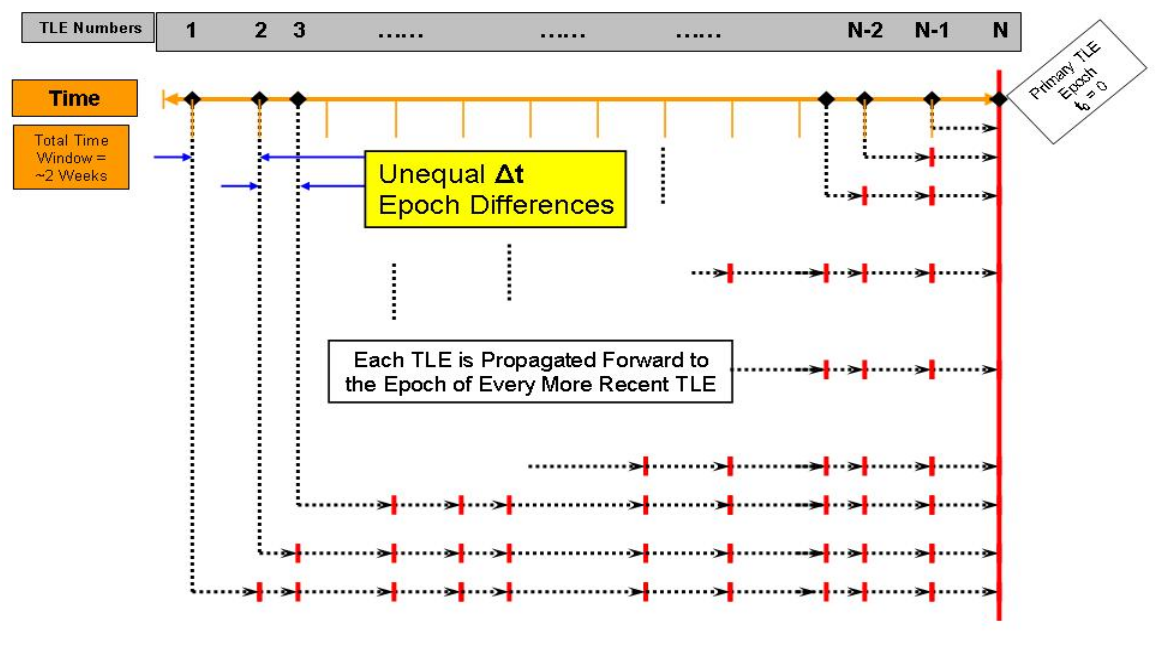
\includegraphics[width=0.8\textwidth]{imagenes/todosOSW}}
  \caption{Esquematizaci\'on del algoritmo para comparar la propagaci\'on de cada TLE del set hacia fechas futuras de los TLE del set. Extra\'ido del trabajo de Osweiler, \citep{osweiler}}.
  \label{fig:todosOSW}
\end{figure}

\begin{figure}[h!]
\centering
  \subfigure[Diferencias ICESAT - ARxCODE]{
    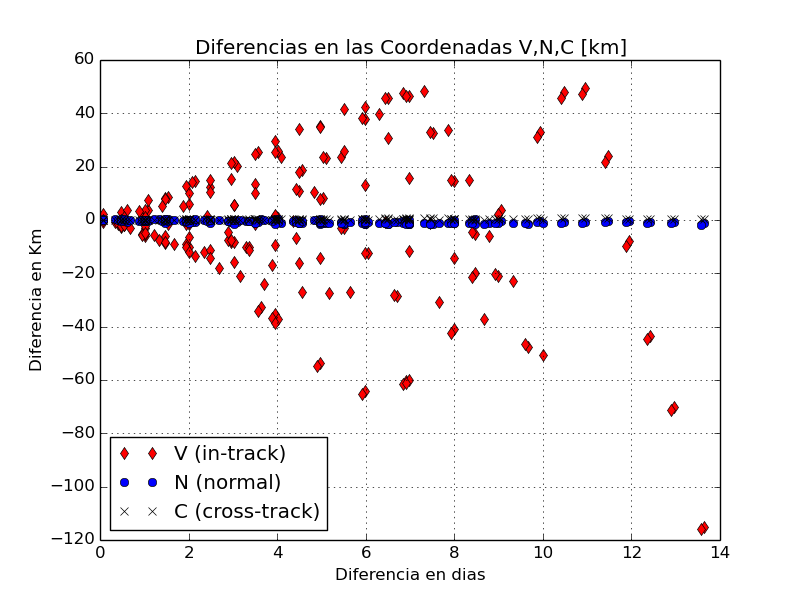
\includegraphics[width=0.48\textwidth]{imagenes/TLEdifTot27642esc52}
  }
  \subfigure[Diferencias ICESAT - Osweiler, \citep{osweiler}]{
    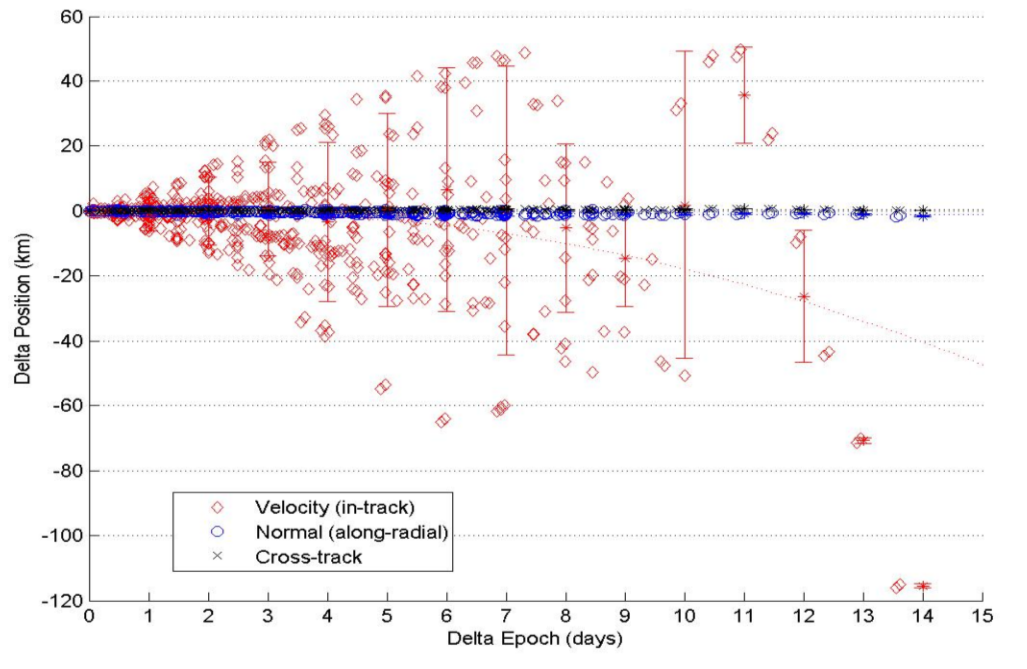
\includegraphics[width=0.48\columnwidth, keepaspectratio]{imagenes/ICESATdifTot}
  }
  \caption{Gr\'afico con Diferencias Totales del escenario ICESAT}
  \label{fig:icesatTot}
\end{figure}

\begin{figure}[h!]
\centering
  \subfigure[Diferencias LAGEOS-1 - ARxCODE]{
    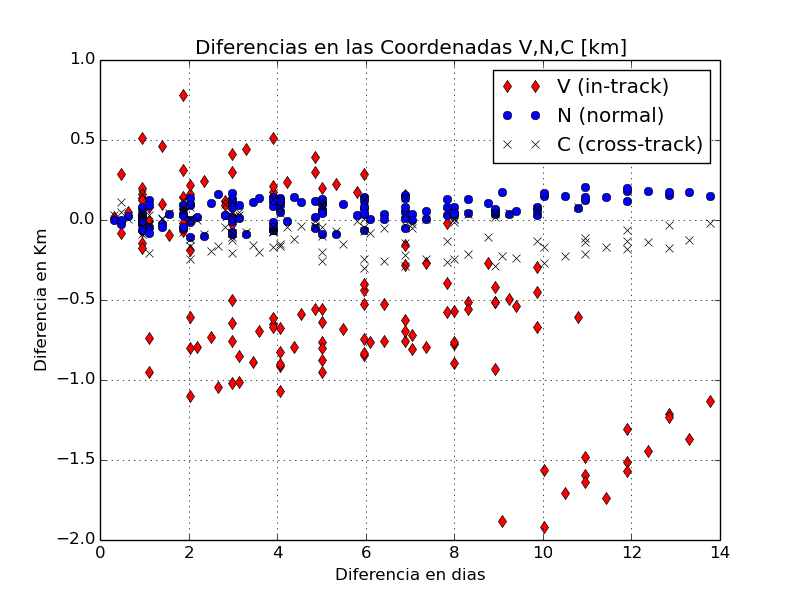
\includegraphics[width=0.48\textwidth]{imagenes/TLEdifTot8820esc11}
  }
  \subfigure[Diferencias LAGEOS-1 - Osweiler, \citep{osweiler}]{
    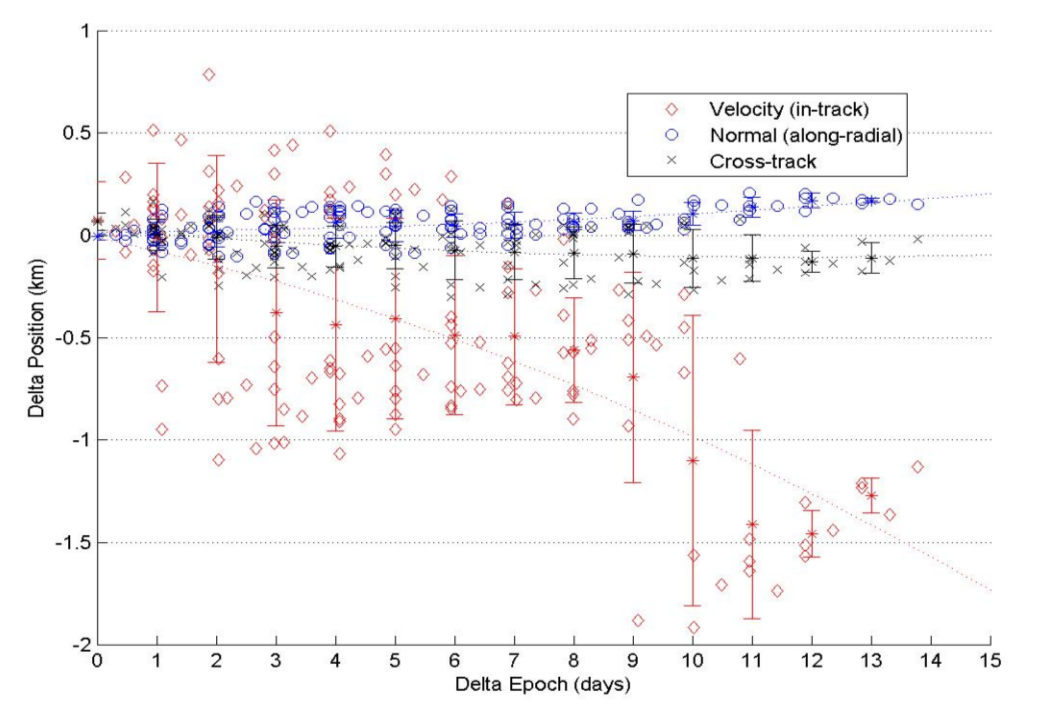
\includegraphics[width=0.48\columnwidth, keepaspectratio]{imagenes/LAGEOSdifTot}
  }
  \caption{Gr\'afico con Diferencias Totales del escenario LAGEOS-1}
  \label{fig:lageosTot}
\end{figure}

Los errores que se observan en la propagaci\'on de TLE, en funci\'on de la cantidad de d\'ias propagados, muestran comportamientos casi id\'enticos.\\

En este estudio, puede apreciarse una clara diferencia en las cotas de los errores, siendo el sat\'elite ICESAT, de menor altura el que muestra errores mayores en un rango de -120 a 60 km, mientras que el LAGEOS, contiene las diferencias entre -2 y 1 km.\\

No obstante, en ambos se distingue, que la componente asociada a la velocidad (V {\it{in-track}}) es la que mayor error acumula en propagaciones m\'as largas. Esto se debe a que el modelo es d\'ebil en cuanto a la perturbaci\'on que introduce la atm\'osfera, directamente vinculada a la velocidad de los objetos para el caso del ICESAT o en cuanto al modelo que describe la presi\'on de radiaci\'on solar en el caso del LAGEOS.\\

Se concluye a partir de esta secci\'on, que ARxCODE implementa el m\'etodo de Osweiler y la construcci\'on de las diferencias de pares correctamente. 

\section{Estudio de errores de TLE con efem\'erides precisas}
\subsection*{Sistema de referencia TOD}
La misi\'on operativa ofrece mediciones propias de sus efem\'erides. En esta secci\'on se muestran los resultados de comparar las posiciones obtenidas mediante los datos p\'ublicos TLE, propagadas con SGP4, contra las efem\'erides precisas.\\ 

En primer lugar fue necesario plasmar las posiciones en el mismo sistema de referencia, ya que los productos del departamento de din\'amica orbital con los que trabajamos ofrecen las posiciones orbitales en el sistema de referencia verdadero de la fecha \ac{TOD}, mientras que los resultados de las propagaciones con el SGP4 se encuentran en el sistema \ac{TEME}. Para poder hacer comparaciones desarrollamos un m\'odulo que transforma las coordenadas y velocidades, del sistema TEME al sistema TOD (Ap\'endice. \ref{App1}).\\

Para la validaci\'on del mismo, utilizamos TLE de la misi\'on y los propagamos con el SGP4. Los resultados que obtuvimos (en el sistema TEME), los transformamos al sistema TOD con el m\'odulo de transformaci\'on desarrollado y luego lo comparamos con los productos del STK, corridos para el mismo TLE y publicados en el sistema TOD que STK ofrece. Las comparaciones se hicieron para propagaciones con paso de 1 minuto a lo largo de todo el dia 01 de Enero de 2013. Los resultados mostraron diferencias menores a los mil\'imetros, de manera que el algoritmo puede usarse sin que incorpore errores significativos  (Tabla \ref{tab:compprecisas}).\\

\begin{table}[!h]
\caption{Comparaci\'on entre ARxCODE y STK de \\la transformaci\'on de TEME a TOD.}
\begin{tabular}{l|c}
  \hline
  Coordenada  X &  0.0003168 [m]\\
  Coordenada Y &  0.0006370 [m]\\
  Coordenada Z &  0.0005133 [m]\\
  \hline
\end{tabular}
\label{tab:compprecisas}
\begin{flushleft}
\small 1 de Enero de 2013, paso 1 minuto.
\end{flushleft}

\end{table}

\subsection*{Estad\'istica de Errores}
Con la certeza de que los datos eran compatibles y pod\'ian ser comparados (ambos se referencian en el sistema TOD), se inici\'o el procesamiento de comparaci\'on de las posiciones de las efem\'erides precisas de la misi\'on y las propagaciones de los TLE, para la estimaci\'on de los errores de la propagaci\'on, (Sec. \ref{subsec:errorProp}).\\

En un pre-procesamiento sobre un periodo amplio de la misi\'on, constatamos que fuera de los intervalos de maniobras por {\it{commissioning}}\footnote{Puesta en \'orbita nominal} o maniobras de rutina, los TLE presentan un error que es {\it{acotado}}, {\it{estable}} y/o modelable. \\

Las comparaciones de las propagaciones de los TLE mostraron significativas aleatoriedades y amplias diferencias en el estudio realizado con los datos correspondientes al a\~no 2012, no obstante los resultados del estudio con datos del a\~no 2013 mostraron la tendencia y estabilidad esperada, con errores m\'aximos del orden de las decenas de kil\'ometros (Fig. \ref{fig:sacd2013}).


\begin{figure}[!h]
\centering
  \textbf{Tendencia Anual 01/01/2013 - 30/08/2013}\par\medskip
  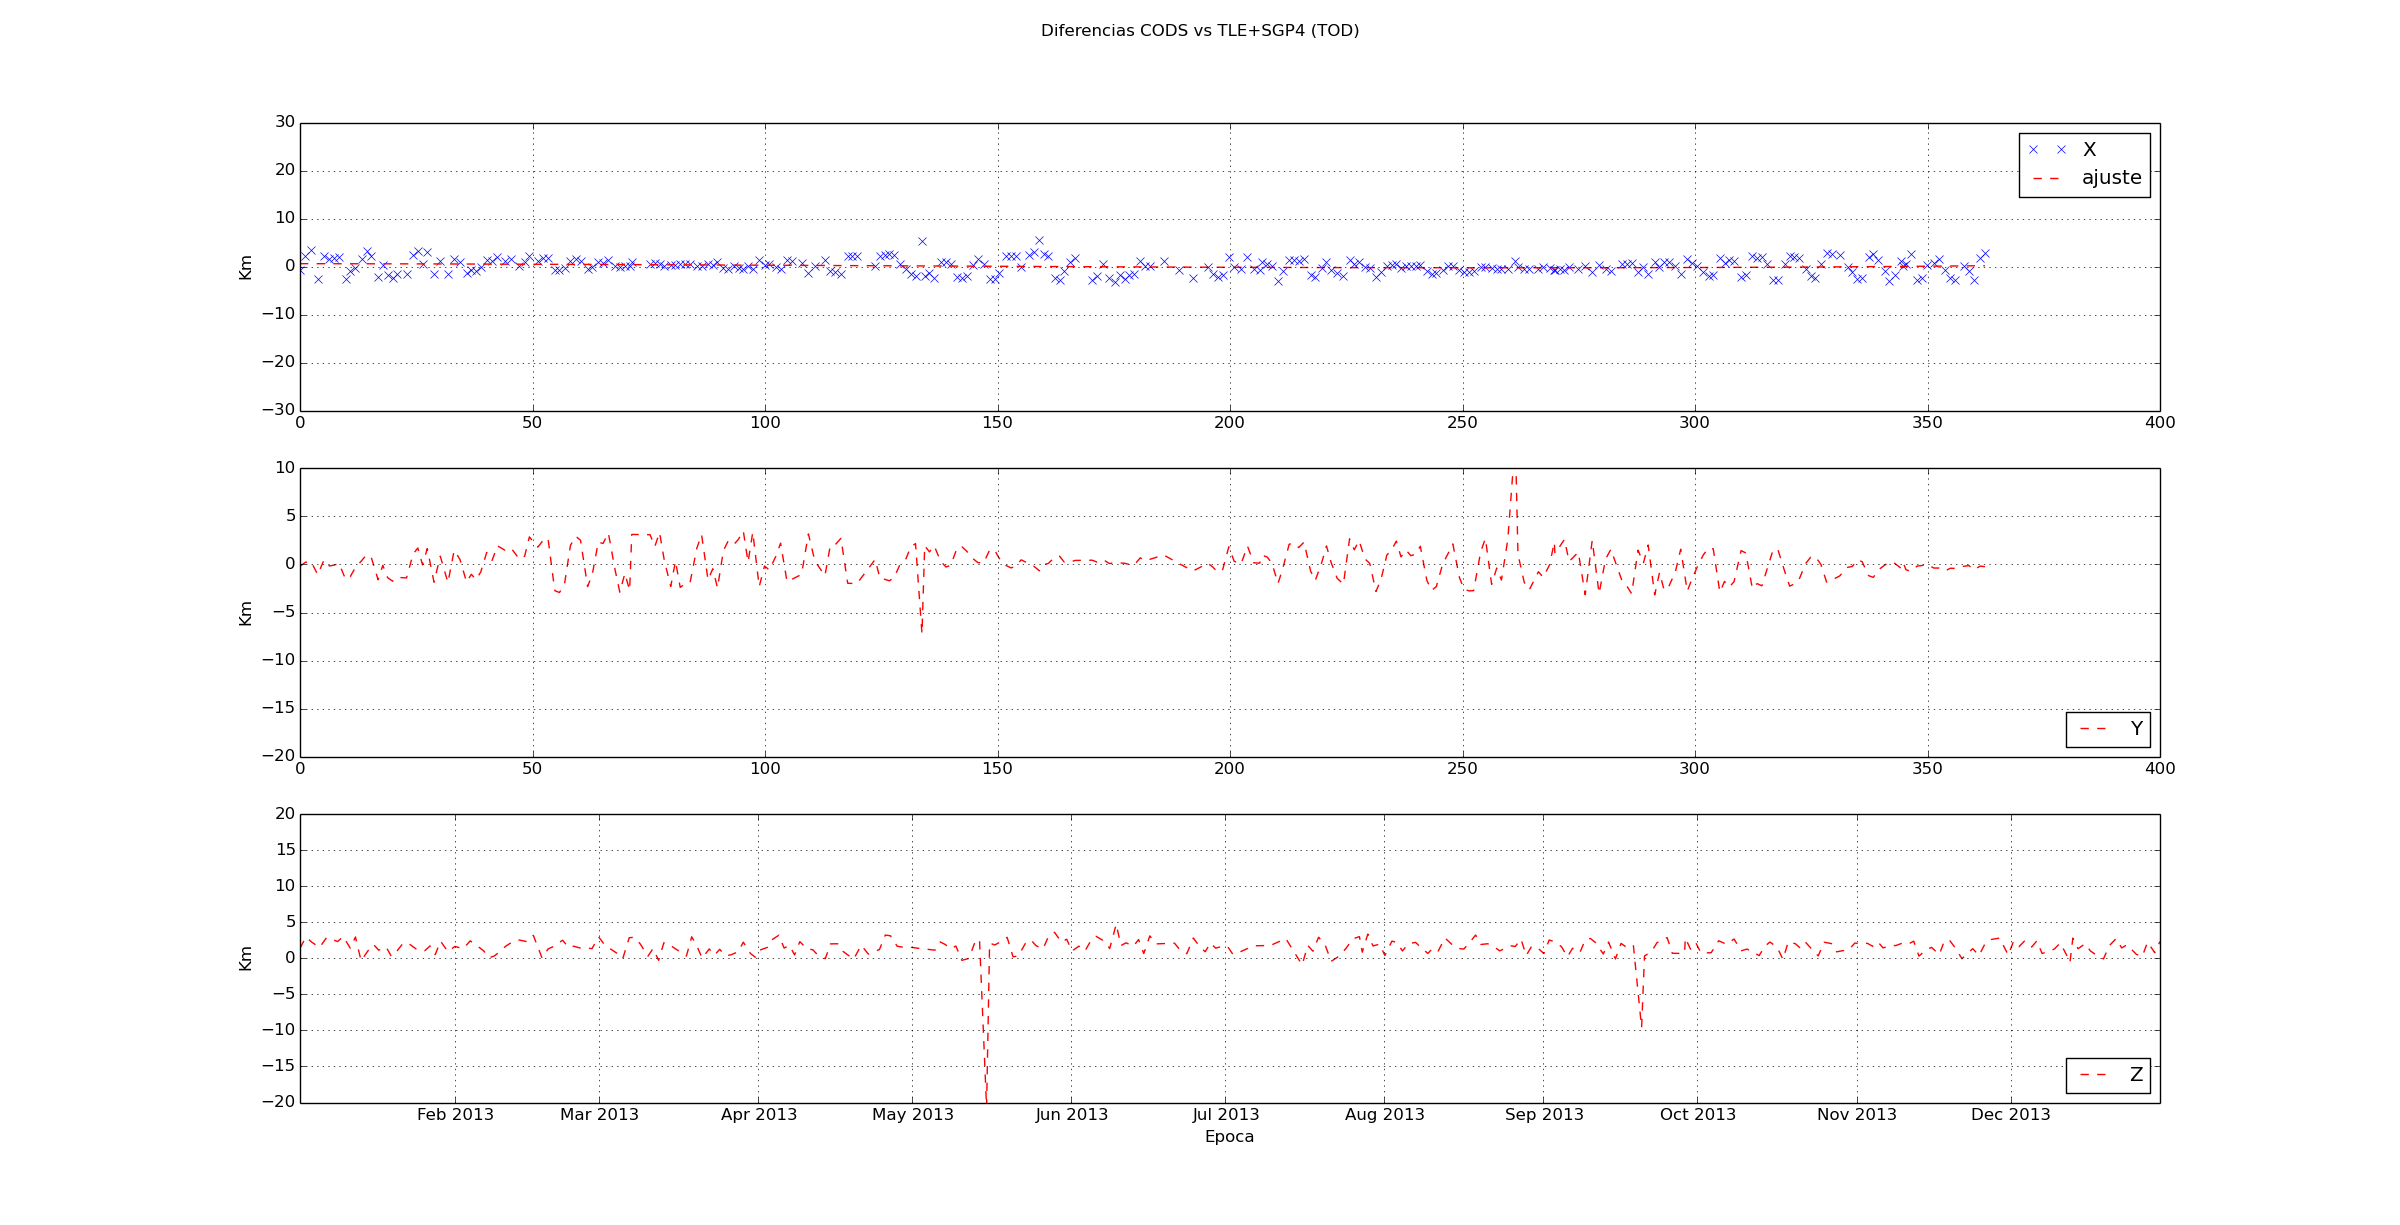
\includegraphics[width=\textwidth]{imagenes/SACD2013todEjesajustados}
  \caption{Tendencia anual de las diferencias contra los datos de din\'amica orbital en coordenadas cartesianas del Sistema TOD}
  \label{fig:sacd2013}
\end{figure}

\subsection*{Generaci\'on de la tabla de propagaci\'on de errores}

Como se explic\'o en la Sec. \ref{subsec:errorProp}, para estimar los errores en la propagaci\'on se propone un m\'etodo que utiliza una tabla (Tabla \ref{tab:resultatabla}), generada a partir de la estad\'istica que resulta de comparar las propagaciones de los TLE de la misi\'on operativa, con las efem\'erides precisas. Las comparaciones se hacen en el periodo de Enero a Junio del a\~no 2013, en intervalos de 1 a 6 d\'ias, con paso 1 segundo.\\

\begin{table}[!h]
\caption[Tabla con los valores medios para la propagaci\'on de errores.]{Valores medios de las varianzas calculadas para la propagaci\'on de errores.\\ Autor\'ia propia.}
\begin{tabular}{lccc}
\hline \hline
\rowcolor{yellow!35}
&$\sigma^{2}_R [km]$ &$\sigma^{2}_T [km]$ &$\sigma^{2}_N [km]$\\
\hline \hline
< 1 d\'ia & 0.05287535953&0.5110606907&0.09802202353\\
\hline
1 d\'ia & 0.03846388969&0.4517572281&0.09807457894\\
\hline
2 d\'ias & 0.02760890529&0.4086434248&0.09904162392\\
\hline
3 d\'ias & 0.01963580775&0.3765098311&0.09022336881\\
\hline
4 d\'ias & 0.01469071678&0.3577884914&0.1182060362\\
\hline
5 d\'ias & 0.01332578794&0.3557767231&0.1264764812\\
\hline
6 d\'ias & 0.01524829841&0.365815954&0.1607439516\\
\hline
\end{tabular}
\label{tab:resultatabla}
\end{table}

Los resultados que se encuentran, no es posible validarlos directamente. No obstante, son comparables a los que proponen Flohrer et al., \citep{flohrer2008assessment}, en la {\it{lookup table}} generada considerando todos los objetos del cat\'alogo al 01 de Enero de 2008 (Fig.  \ref{fig:flohrer}). Los valores de las desviaciones est\'andar que resultan del m\'etodo propuesto son menores casi en un orden de magnitud a las tablas gen\'ericas que publican Flohrer et al., \citep{flohrer2008assessment}, esto es de esperar, ya que los estudios de la publicaci\'on son m\'as abarcativos y gen\'ericos.\\

\begin{figure}[!h]
  \centering
  \fbox{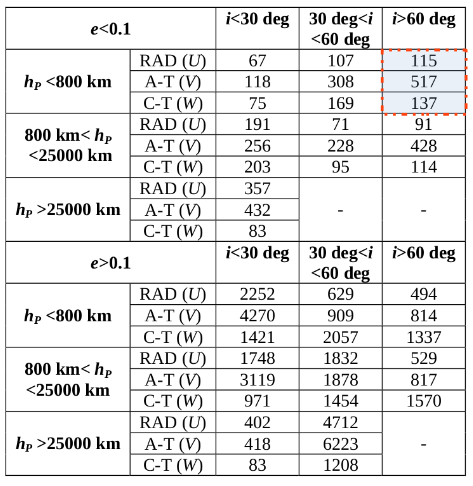
\includegraphics[width=0.6\textwidth]{imagenes/flohrertabla}}
  \caption{{\it{Look-up table}} [metros] de los resultados promediados del an\'alisis del cat\'ologo completo al 01 de Enero de 2008, de los errores en las coordenadas UVW, clasificados por excentricidad, inclinaci\'on y altura. Se resaltan en celeste las celdas correspondientes a la configuraci\'on de la misi\'on operativa que se utiliz\'o en este trabajo. Extra\'ido de Flohrer et al., \citep{flohrer2008assessment}}.
  \label{fig:flohrer}
\end{figure}

% \begin{itemize}
%  \item Klinkrad Tabla para 14 misiones.
%  \item Paper del research gate
%  \item Peterson?!
% \end{itemize}
% 
% FINALIZAR CON COMPARACI\'ON TLE vs TLE. 

\section{C\'alculo de la Probabilidad de Colisi\'on}

El c\'alculo de la PoC implementa la expresi\'on presentada por Lei-Chen, \citep{leichen}.


\subsection*{Comparaci\'on de los resultados con la resoluci\'on de la integral}
Con el objeto de verificar los c\'alculos que se realizan en el m\'odulo, se toman como datos iniciales, los valores publicados por el propio autor Lei-Chen, \citep{leichen}, y se calcula la PoC, tanto para la expresi\'on anal\'itica como la integral. Para esta \'ultima se utiliza la biblioteca {\it{scipy.integrate}}  de python.\\

De las expresiones para el c\'alculo de la PoC (Eq. \ref{eq:pocintegral} y Eq. \ref{eq:pocexpress}), se desprende que ser\'an necesarios los datos: ($\mu_{x}, \mu_{y}$), ($\sigma_{x}, \sigma_{y}$), $r_{a}$.\\

Se tomaron los datos que utiliza Lei-Chen en el ejemplo para el caso de las \'orbitas circulares y se calcul\'o la PoC a partir de la expresi\'on expl\'icita y realizando la integral.\\

\begin{minipage}[t]{0.28\textwidth}
{\bf{Valores iniciales.}}\\

\begin{tabular}{|lc|}
\hline
 Dato & valor \\
\hline
$\mu_{x}$ & 0.031731 [km]\\
$\mu_{y}$ & 0.697294 [km]\\
$\sigma_{x}$ & 0.0430576\\
$\sigma_{y}$ & 0.2941297\\
$r_{a}$ & 0.01 [km]\\
\hline
\end{tabular}
\end{minipage}
\begin{minipage}[t]{0.7\textwidth}
\begin{mdframed}[
        linecolor=red,linewidth=2pt,% 
        frametitlerule=true,% 
        apptotikzsetting={\tikzset{mdfframetitlebackground/.append style={%
            shade,left color=white, right color=blue!20}}}, 
        frametitlerulecolor=blue,
        frametitlerulewidth=1pt, innertopmargin=\topskip,
        frametitle={Probabilidad de Colisi\'on},
        outerlinewidth=1.25pt
    ]
\large
\captionof{table}{Resultados Comparativos del c\'alculo de la PoC.}
\begin{tabular}{|l|l|l|}
  \hline
 Te\'orico & Expresi\'on & Valor de la Integral\\
 \hline
 1.8079750e-04 & 1.8079124e-04 & 1.8071110e-04\\
 \hline
\end{tabular}
\label{tab:poccomp}
\end{mdframed}
\end{minipage}

\vspace{0.5cm}
Como se observa en el recuadro de las probabilidades de colisi\'on (Tabla \ref{tab:poccomp}); las f\'ormulas implementadas coinciden con el valor de la bibliograf\'ia hasta el cuarto d\'igito significativo de la expresi\'on.\\

En este punto se confirma que, una vez que se obtiene: $\mu_{x}$, $\mu_{x}$, $\sigma_{x}$, $\sigma_{y}$ y el radio de colisi\'on $r_{a}$, ya puede calcularse la PoC. 
Ahora resta verificar, paso a paso c\'omo llegar de los inputs de ARxCODE, a estos par\'ametros que se introducen en de las ecuaciones. \\

\subsection*{C\'alculos previos}

Una vez determinadas la posici\'on relativa de los objetos en el sistema RSW o RTN en el TCA, la proyecci\'on al plano para \'orbitas circulares, no representa mayores problemas, como se detall\'o en la Sec. \ref{subsec:pocsimp}.\\

Pero es importante verificar, que a partir de las posiciones inerciales de los objetos en el TCA, las transformaciones de la distancia relativa de los mismos al sistema RSW, coincide.
Para ello, vamos a utilizar las posiciones de los objetos del ejemplo de la bibliograf\'ia (Tabla \ref{tab:vectejemplo}) y transformarlas con el m\'odulo de transformaci\'on {\it{sisRic}} del paquete {\it{SistReferencia.SistdeCoordenadas}} para corroborar los resultados.
\\

\begin{table}[!h]
\caption{Vectores de Posiciones Inerciales al momento TCA.}
\begin{tabular}{lcccccc}
\hline
Objeto & x [km] & y [km] &z[km] &vx [km] &vy [km] &vz [km]\\
\hline
Obj1 & 1457.273246 &1589.568484&6814.189959&7.001731&2.439512&0.926209\\
Obj2 & 1457.532155&1588.932671&6814.316188&3.578705&6.172896&2.200215\\
\hline
\end{tabular}
\label{tab:vectejemplo}
\begin{flushleft}
\small {\it{Nota.}} Extra\'idos del ejemplo de la bibliograf\'ia \citep{leichen}.
\end{flushleft}
\end{table}

\begin{table}[!h]
\caption{Comparaci\'on entre el m\'odulo {\it{sisRic}} de autor\'ia propia \\y los datos de Lei-Chen \citep{leichen}.}
\begin{tabular}{lccc}
\hline
Resultados seg\'un & R [km] & S [km] & W[km] \\
\hline
Lei Chen & 0.031731& 0.436476&0.543785\\
ARxCODE & 0.031797& 0.462295 &0.522013
\\
\hline
\end{tabular}
\label{tab:rswcomp}
\end{table}

Estos resultados que se publican en la Tabla \ref{tab:rswcomp}, se logran en una transformaci\'on en la que se considere al Obj2 como origen de la referencia. Los mismos muestran una coincidencia del orden de las decenas de metros, aceptable para estas estimaciones.
No obstante, contando s\'olo con la informaci\'on de los vectores de posici\'on al momento del m\'aximo acercamiento, no es posible verificar el m\'etodo de Osweiler de la construcci\'on de la matriz de covarianza para este ejemplo de la bibliograf\'ia.\\

\subsection*{Validaci\'on {\it{end-to-end}}}
Hasta este punto, se han validado cada uno de los procesos por separado.
Resta hacer pruebas desde el origen, es decir a partir de identificar los objetos y el TCA, correr los procesamientos de ARxCODE y obtener los resultados de la PoC.
A tal fin, fue necesario conseguir registros que contuvieran la informaci\'on completa de una situaci\'on de encuentro.\\

Por un lado tuvimos acceso a correos electr\'onicos de alerta p\'ublicos en internet, y por otro a CDM tambi\'en p\'ublicos\footnote{https://cwe.ccsds.org/moims/docs/Forms/AllItems.aspx?RootFolder=\%2Fmoims\%2Fdocs\%2FMOIMS-NAV\%2FDraft\%20Documents\%2FConjunction\%20Data\%20Message\%20\%28CDM\%29}, pero ninguno de esos datos se corresponden con la misi\'on operativa, cuyas efem\'erides precisas analizamos y utilizamos en la construcci\'on del modelo estad\'istico de propagaci\'on de errores.
As\'i mismo, ni los correos encontrados ni los CDM descargados contienen informaci\'on de la PoC asociada al encuentro. \\

Finalmente se analizaron casos presentados en libros o publicaciones, que contienen los datos iniciales necesarios para disparar el procesamiento y valores de la PoC.\\


\subsubsection*{Validaci\'on con correos electr\'onicos de alerta p\'ublicos}

El proceso de validaci\'on utilizando los correos electr\'onicos obtenidos en la web, consiste de extraer de los correos los identificadores de norad de ambos objetos y el TCA asociado al encuentro. A partir de all\'i se calcula la m\'inima distancia total, o sea el m\'odulo de la misma, y  en componentes en el sistema RTN y finalmente la PoC.
Dado que el TCA que se publica en los correos no tiene informaci\'on de los segundos, se realiza una primera estimaci\'on, y luego se profundiza en an\'alisis de la situaci\'on.\\

Formato de los correos electr\'onicos:\\
\begin{center}
\fbox{\parbox[b]{0.8\linewidth}{
The United States Joint Space Operations Center (JSpOC) has identified a\\
predicted conjunction between DELFI C3 (SCC\# 32789) and SCC\# 23657.\\

Primary Object: DELFI C3 (SCC\# 32789)\\
Secondary Object: SCC\# 23657\\
Time of Closest Approach: 15 JUL 2012 21:21 UTC \\

Overall miss distance: 760 meters\\
Radial (dU) miss distance: -186 meters\\
In-Track (dV) miss distance: -389 meters\\
Cross-track (dW) miss distance: -626 meters\\

Primary Radial Error (U): 38 meters\\
Primary In-track Error (V): 1388 meters\\
Primary Cross-track Error (W): 11 meters\\

Secondary Radial Error (U): 8 meters\\
Secondary In-track Error (V): 338 meters\\
Secondary Cross-track Error (W): 2 meters\\
}}
\end{center}

{\bf{Nota:}} Los los correos electr\'onicos no informan los segundos del TCA. Fue necesario primero hacer una primera estimaci\'on m\'as precisa del TCA del encuentro y luego volver a procesar incorporando los segundos. 

Se listan a continuaci\'on los cinco correos electr\'onicos cuyos datos fueron procesados con ARxCODE. La Figura \ref{fig:tablamails}, muestra el resumen de la informaci\'on de todos los correos electr\'onicos. 
\begin{figure}[!h]
  \centering
  \fbox{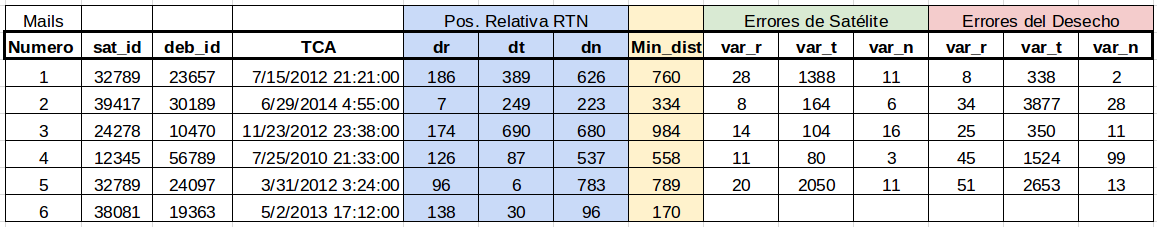
\includegraphics[width=\textwidth]{imagenes/tablamails}}
  \caption{Contenido de los correos electr\'onicos utilizados para comparar los resultados.}
  \label{fig:tablamails}
\end{figure}

A partir de esa informaci\'on se carg\'o manualmente el identificador de NORAD del sat\'elite (sat\_id), el identificador de NORAD del desecho (deb\_id), y el TCA de cada situaci\'on; en un primer paso se utiliz\'o ARxCODE para obtener el valor de los segundos del TCA. Luego se propag\'o para el TCA que inclu\'ia los segundos, con pasos de propagaci\'on distintos, en un caso cada un segundo (Tabla \ref{tab:mails1seg}) y en otro caso para un paso menor, de cien mil microsegundos (Tabla \ref{tab:mails100mseg}).\\

\begin{table}[!h]
\caption{ARxCODE a partir de correos electr\'onicos\\ Propagaciones cada 1 segundo - (Radio de colisi\'on $r_{a}=0.01$ km)}
\resizebox{17cm}{!}{
\begin{tabular}{ccrrrrr}
 \hline \hline
 \# & TCA arx & $\Delta R_{arx}$ [km] & $\Delta T_{arx}$ [km] & $\Delta N_{arx}$ [km] & Min Dist. arx [km] & PoC arx\\
 \hline \hline
 1 & 2012-07-15 21:21:51 & 0.147 & 2.749 &  2.287 & 3.579 & 4e-06 \\
 
 2 & 2014-06-29 04:55:59 & 0.081 & 3.921 & 2.002 & 4.403 & 0.0 \\
 
 3 & 2012-11-23 23:38:42 & 0.300 & 1.668 & 0.841 & 1.892 & 0.0 \\

 4 & 2013-03-31 03:25:45 & 68.07& 1.318 & 426.1 & 431.5 & 0.0 \\

 5 & 2013-05-02 17:12:04 & 19.07 & 489.6 & 142.7 & 510.3& 0.0 \\
 \hline
\end{tabular} }
\label{tab:mails1seg}
\end{table}


\begin{table}[!h]
\caption{ARxCODE a partir de correos electr\'onicos\\ Propagaciones cada 100.000 microsegundos - (Radio de colisi\'on $r_{a}=0.01$ km)}
\resizebox{17cm}{!}{
\begin{tabular}{ccrrrrr}
 \hline \hline
 \# & TCA arx & $\Delta R_{arx}$ [km] & $\Delta T_{arx}$ [km] & $\Delta N_{arx}$ [km] & Min Dist. arx [km] & PoC arx\\
 \hline \hline
 1 & 2012-07-15 21:21:51.3 & 0.142 & 0.512 &  0.254 & 0.589 & 4e-06 \\
 
 2 & 2014-06-29 04:55:59.1 & 0.082 & 3.253 & 2.745 & 4.258 & 0.0 \\
 
 3 & 2012-11-23 23:38:42.1 & 0.258 & 0.936 & 1.595 & 1.867 & 1.7e-05 \\
 
 4 & 2013-03-31 03:25:45.1 & 68.07 & 0.194 & 426.1 & 431.5 & 0.0 \\
 
 5 & 2013-05-02 17:12:02.9 & 20.17 & 504.1 & 146.8 & 525.4 & 0.0\\
 \hline
\end{tabular} }
\label{tab:mails100mseg}
\end{table}

\begin{table}[!h]
\caption{M\'inimas distancias de acercamiento para distintos pasos de propagaci\'on y\\ resultados de los los correos electr\'onicos.}
%\resizebox{8cm}{!}{
\begin{tabular}{cccc}
 \hline \hline
  \rowcolor{lightgray}
 \# & Dist (1 seg) [km] & Dist (100 mil $\mu$ seg) [km] & Dist. correo\\
 \hline \hline
 1 & 3.579 &  0.589 &  0.760  \\
 
 2 & 4.403 & 4.258 & 0.334  \\
 
 3 & 1.892 & 1.867 & 0.984 \\
 
 4 & 431.5 & 431.5 & 0.789 \\
 
 5 & 510.3 & 525.4 & 0.170 \\
 \hline
\end{tabular} %}

\label{tab:mailsMinD}
\end{table}

Como puede apreciarse en la Tabla \ref{tab:mailsMinD} de las comparaciones, los distintos pasos de propagaci\'on no modifican los resultados significativamente, salvo en el primer caso. De manera que resulta importante revisar instancias previas, es decir analizar las matrices de error de cada objeto generadas por ARxCODE (Fig. \ref{fig:tablaMAmails}).\\

 \begin{figure}[!h]
  \centering
  \fbox{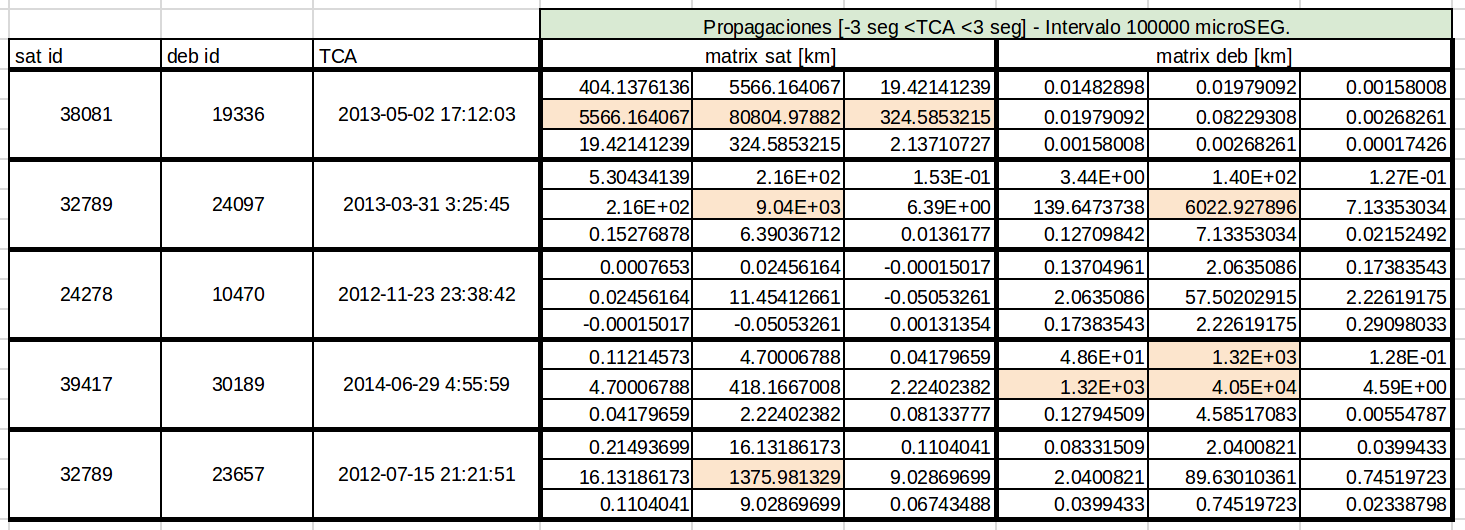
\includegraphics[width=\textwidth]{imagenes/tablaMAmails}}
  \caption{Tabla con las matrices de covarianza calculadas por ARxCODE (m\'etodo de Osweiler) para la misi\'on y el desecho. Se resaltan los valores que con errores grandes}
  \label{fig:tablaMAmails}
\end{figure}

Se observa, que las matrices calculadas para introducir en el c\'alculo del encuentro de ARxCODE, introducen errores muy grandes y los elementos de su diagonal, correspondientes a las varianzas en cada una de las componentes RTN, son mucho mayores a las que se indican en los mails.\\

De estos resultados se desprende que los valores publicados en los mails, son m\'as precisos a los que se pueden lograr con ARxCODE y seguramente han sido calculados con datos observacionales de rastreo m\'as precisos que la informaci\'on orbital que ofrecen los TLE. 

\subsubsection*{Validaci\'on con CDM p\'ublicos}

Se listan a continuaci\'on los seis CDM cuyos datos fueron procesados con ARxCODE (Fig. \ref{fig:cdmsproc}). A partir de esa informaci\'on se carg\'o manualmente el identificador de NORAD del sat\'elite (sat\_id), el identificador de NORAD del desecho (deb\_id), el TCA de cada situaci\'on. Se calcul\'o la m\'inima distancia y la PoC, con pasos de propagaci\'on distintos, en un caso cada un segundo (Tabla \ref{tab:cdmsproc1seg}) y en otro caso para un paso menor, de cien mil microsegundos (Tabla \ref{tab:cdmsproc100mseg}).\\
 
 \begin{figure}[!h]
  \centering
  \fbox{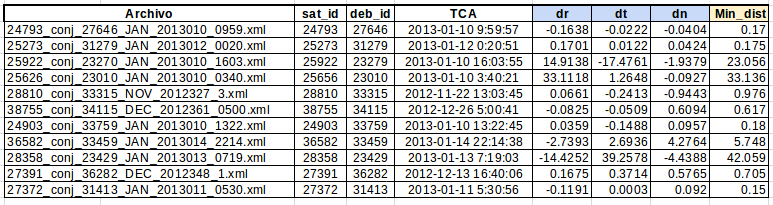
\includegraphics[width=\textwidth]{imagenes/tablaCDM}}
  \caption{Contenido de los CDM utilizados para comparar los resultados.}
  \label{fig:cdmsproc}
\end{figure}
 
 \begin{table}[!h]
  \caption{ARxCODE a partir de los CDM \\ Propagaciones cada 1 segundo - (Radio de colisi\'on $r_{a}=0.01$ km)}
 \centering
 \resizebox{17cm}{!}{
\begin{tabular}{ccrrrrr}
 \hline \hline
 \# & TCA arx & $\Delta R_{arx}$ [km] & $\Delta T_{arx}$ [km] & $\Delta N_{arx}$ [km] & Min Dist. arx [km] & PoC arx\\
 \hline \hline
 1 & 2013-01-10 09:59:57 &0.295626&1.358542&1.321294&1.918033& 1.4e-05 / 1.4e-05\\
 
 2 & 2013-01-12 00:20:51 &0.405629&4.127385&1.632732&4.457091&0.0 / 0.0\\
 
 3 & 2013-01-10 13:22:45 & 0.382972 & 1.173174  & 1.316177 & 1.804252 & 8e-06\\

 4 & 2013-01-11 05:30:56 & 0.01038& 1.276203& 0.648991&1.431779&0.0\\
 
 5 & 2012-11-22 13:03:45.0 & 0.027395 & 4.661372 & 0.332569 & 4.673301 & 1.4e-05/1.4e-05 \\
 
 6 & 2012-12-26 05:00:41 & 0.183897& 4.661359&0.02668&4.665061& 0.0 / 0.0\\
 \hline
 \end{tabular} }

 \label{tab:cdmsproc1seg}
 \end{table}
 
\begin{table}[!h]
 \caption{ARxCODE a partir de los CDM \\ Propagaciones cada 100.000 microsegundos - (Radio de colisi\'on $r_{a}=0.01$ km)}
\centering
 \resizebox{17cm}{!}{
\begin{tabular}{ccrrrrr}
 \hline \hline
 \# & TCA arx & $\Delta R_{arx}$ [km] & $\Delta T_{arx}$ [km] & $\Delta N_{arx}$ [km] & Min Dist. arx [km] & PoC arx\\
 \hline \hline
 1 &2013-01-10 09:59:57  &0.295626&1.358542& 1.321294&1.918033&1.4e-05 \\
 
 2 & 2013-01-12 00:20:51.3 &0.401158&0.140306&0.218037&0.477654&6.1e-05\\
 
 3 & 2013-01-10 13:22:45.2 & 0.382381 &0.288759& 0.043842&0.481165&9e-06\\
 
 4 &2013-01-11 05:30:55.9&0.016754 &0.215364 &0.573953&0.613257&0.0\\
 
 5 & 2012-11-22 13:03:44.7 & 0.023908 & 0.436662& 0.758981 & 0.875955 & 2e-05 \\
 
 6 & 2012-12-26 05:00:40.7 & 0.183162& 0.1859&0.417861&0.492661& 1.24e-04\\
 \hline
 \end{tabular} }
 \label{tab:cdmsproc100mseg}
 \end{table}

 \begin{table}[!h]
 \caption{M\'inimas distancias de acercamiento para distintos pasos de propagaci\'on \\ y resultados de los CDM. (Radio de colisi\'on $r_{a}=0.01$ km)}
\label{tab:cdmsMinD}
\begin{tabular}{lccc}
 \hline \hline
  \rowcolor{lightgray}
 \# & Dist (1 seg) [km] & Dist (100 mil $\mu$ seg) [km] & Dist. CDM\\
 \hline \hline
 1 & 1.918 &  1.918&  0.170 \\
 
 2 & 4.457 & 0.477 & 0.175  \\

 3 & 1.804 & 0.481 & 0.180\\
 
 4 & 1.431 & 0.613 & 0.150\\
 
 5 & 4.665 & 0.875 & 0.976 \\
 
 6 & 4.665 & 0.492 & 0.617\\
 \hline
\end{tabular} 
\end{table}

Para estos \'ultimos procesamientos es notoria la diferencia que se produce cuando se incrementa el paso de propagaci\'on al orden de los cien mil microsegundos; logrando as\'i que los valores calculados por ARxCODE para las m\'inimas distancias se aproximen al valor que publican los CDM.\\

No se pudo identificar a qu\'e se debe esta distinci\'on entre las mejoras que se logran en los CDM, que no se logran en la informaci\'on que proviene de los correos electr\'onicos, aunque probablemente se deba a la incerteza en el TCA que introducen los correos al no informar el TCA con precisi\'on del segundo.\\

\subsubsection*{Validaci\'on con bibliograf\'ia que incluye PoC}

En el cap\'itulo ocho de su libro, Klinkrad \citep{Klinkrad}, publica una tabla que contiene siete situaciones de encuentros de riesgo para las misiones ENVISAT y ERS-2. De esos escenarios s\'olo se han podido reproducir dos, ya que no fue posible identificar los c\'odigos de NORAD de los desechos involucrados en el resto de los encuentros.
Para esos dos escenarios, se calcularon la m\'inima distancia y la PoC, y se compararon los resultados con los publicados en el libro de Klinkrad (Tabla \ref{tab:escenariosKlinkrad}).\\

 \begin{table}[!h]
 \caption{Comparaci\'on de ARxCODE con los resultados de Klinkrad \citep{Klinkrad}.\\ Paso de propagaci\'on, cien mil $\mu$s y radio de colisi\'on $r_{a}=0.01$ km}
\resizebox{17cm}{!}{
\begin{tabular}{lccccccc}
 \hline \hline
  \rowcolor{lightgray}
 \multirow{2}{*}{\#} & sat id & deb id & TCA & Min Dist [km] & Min Dist [km]& PoC  & Poc \\
 \rowcolor{lightgray}
 &&&& (Klinkard)&ARxCODE &(Klinkard)&ARxCODE\\
 \hline
 1 & 27386 &  12442&  2004-09-02 19:14:11 &1.297& 1.443&2.186e-04  &3.1e-05 \\
 
 2 & 23560 & 16681 & 2004-09-29 23:56:02 &0.067&0.557&1.546e-04& 2e-05 \\
 \hline
\end{tabular} }
\label{tab:escenariosKlinkrad}
\end{table}

En un mismo sentido, se utilizaron los valores publicados en el trabajo de Xu y  Xiong, \citep{xu2014method}, donde  se presentan las estimaciones de la m\'inima distancia y la Poc, utilizando un m\'etodo general y el m\'etodo desarrollados por ellos (Tabla \ref{tab:escenariosxx}).\\

 \begin{table}[!h]
 \caption{Comparaci\'on de ARxCODE con los resultados de  Xu \& Xiong \citep{xu2014method}.\\ Paso de propagaci\'on cien mil $\mu$s y radio de colisi\'on $r_{a}=0.01$ km.  }
\centering
\resizebox{17cm}{!}{
\begin{tabular}{lcccccccc}
 \hline \hline
  \rowcolor{lightgray}
 \multirow{2}{*}{\#} & sat id & deb id & TCA & Min Dist [km] & Min Dist [km]& Poc & PoC  & Poc \\
 \rowcolor{lightgray}
 &&&& (Xu\&Xiong)&ARxCODE &(General)&(Xu\&Xiong)&ARxCODE\\
 \hline
 1 & 25415 &  31445&  2013-03-18 14:44:34 &0.115&0.951 & 1.24e-05 &1.52e-05 &8e-06\\
 
 2 & 20737 & 20738 &2013-03-17 10:39:31 &0.104&0.0365&1.706e-06& 2.15e-06& 6.06e-04\\
 
 3 & 27939 & 31588 &2013-03-16 13:46:21 &0.098&1.048&3.01e-05&3.51e-05&9e-06 \\
 
 4 & 11308 & 32315 &2013-03-15 03:02:16 &0.094&0.263&1.8e-05& 2.05e-05& 1.04-03\\
 
 5 & 17583 & 37442 &2013-03-16 14:02:50 &0.039& (*)&9.39e-05& 1.88e-04& (*) \\
 \hline
\end{tabular} }
\begin{flushleft}\tiny{(*) No se obtuvieron TLEs del desecho para la fecha publicada.}\end{flushleft}
\label{tab:escenariosxx}
\end{table}

En las comparaciones se observa que los resultados de ARxCODE distan en centenares de metros con los datos encontrados en la bibliograf\'ia para la determinaci\'on de la m\'inima distacia, y en uno o dos \'ordenes de magnitud en el c\'alculo de la PoC.
Mientras que para el caso de las m\'inimas distancias, los valores de ARxCODE son siempre superiores a los valores d e la bibliograf\'ia, en el caso de las PoC no hay un comportamiento repetido, siendo que para algunos casos en por mucho mayor al valor de la bibliograf\'ia y en otros caso menor.\\ 

\subsubsection*{C\'alculo de la PoC en funci\'on del radio de colisi\'on}

Las \'ultimas situaciones; trabajos de Klinkrad \citep{Klinkrad} y Xi \& Xiong \citep{xu2014method}; que se utilizaron para comparar los resultados de ARxCODE, dan informaci\'on de los objetos involucrados y del TCA, no obstante, no se informa sobre la estimaci\'on que han hecho para el radio de colisi\'on.\\

A continuaci\'on las Figuras \ref{fig:pocvsraEsc4} y \ref{fig:pocvsraEsc5} muestran los valores de la PoC calculados con ARxCODE en funci\'on del radio de colisi\'on elegido, para los escenarios del libro de Klinkrad descriptos previamente.\\

Como puede verse, el c\'alculo de la PoC resulta muy sensible al radio de colisi\'on considerado. Se desconoce cu\'al es el radio utilizado por Klinkrad, pero puede distinguirse que en un rango de radios de $r_{a}=0.001$ hasta $r_{a}=0.03$ kil\'ometros, se ubican las soluciones de la bibliograf\'ia.\\

Se adjuntan en el Ap\'endice \ref{App2}, los gr\'aficos an\'alogos para los resultados del trabajo de Xu \& Xiong.\\

 
\begin{figure}[!h]
  \centering
  \fbox{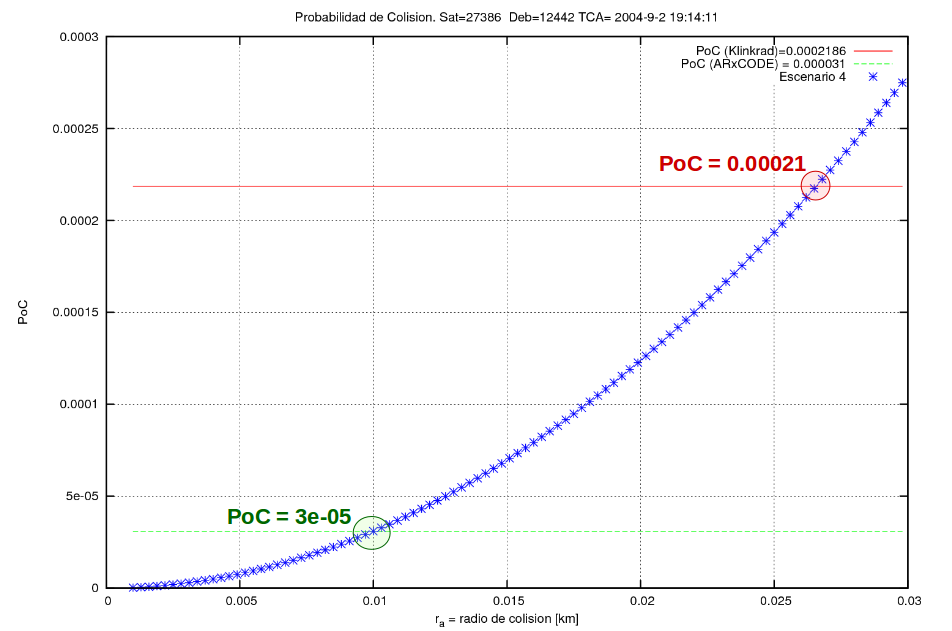
\includegraphics[width=\textwidth]{imagenes/klinkradEsc4mod}}
  \caption{An\'alisis de la PoC en funci\'on del radio de colisi\'on. La l\'inea roja indica el valor de la PoC calculada por Klinkrad \citep{Klinkrad} y el c\'irculo se\~nala el cruce con el radio $r_{a}$ correspondiente. La l\'inea verde indica la PoC calculada por ARxCODE para un $r_{a}=0.01$ km. (Escenario 1)}
  \label{fig:pocvsraEsc4}
\end{figure}

\begin{figure}[!h]
  \centering
  \fbox{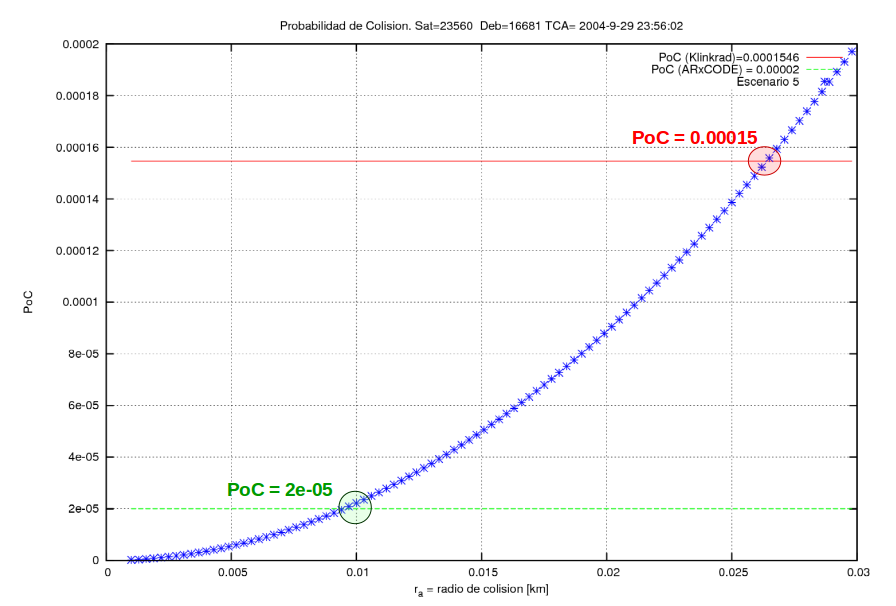
\includegraphics[width=\textwidth]{imagenes/klinkradEsc5mod}}
  \caption{An\'alisis de la PoC en funci\'on del radio de colisi\'on. La l\'inea roja indica el valor de la PoC calculada por Klinkrad \citep{Klinkrad} y el c\'irculo se\~nala el cruce con el radio $r_{a}$ correspondiente. La l\'inea verde indica la PoC calculada por ARxCODE para un $r_{a}=0.01$ km. (Escenario 2)}
  \label{fig:pocvsraEsc5}
\end{figure}

\newpage
\section{An\'alisis} 
 A partir de estos resultados, se desprenden los siguientes an\'alisis:\\
 
 \begin{itemize}
  \item Las funcionalidades para la conexi\'on con NORAD para la descarga de TLE, y las propagaciones que se realizan de los mismos, funcionan correctamente.\\
  \item El m\'etodo de Osweiler \citep{osweiler} para la generaci\'on de la matriz de covarianza, resulta con diferencias del orden de los cent\'imetros respecto de los valores publicados. Resultado m\'as que aceptable dado que las \'orbitas m\'as precisas que se consideran en este trabajo tienen errores del orden de 20 metros.\\
  \item El estudio de los errores en funci\'on de la cantidad de d\'ias que se propaguen los TLE, coincide con los resultados publicados por Osweiler \citep{osweiler} y respeta los valores esperados, de acuerdo a los efectos perturbativos y las caracter\'isticas de las \'orbitas de los sat\'elites analizados.\\
  \item Las tendencias en los errores que se obtienen al comparar las propagaciones de los TLE con las efem\'erides precisas a lo largo del a\~no 2013, mostraron un comportamiento estable y acotado, salvo outliers, como se esperaba. Con cotas superiores de decenas de kil\'ometros.\\
  \item La metodolog\'ia utilizada para estimar errores en la propagaci\'on, mostr\'o resultados comparables y a\'un mejores que los propuestos por Flohrer et al., \citep{flohrer2008assessment}.
  \item Las transformaciones al sistema de referencia RTN tienen diferencias del orden de las decenas de metros con las publicadas en el ejemplo de Lei-Chen \citep{leichen}.\\
  \item No se cuenta con datos para poder validar las proyecciones de la posici\'on relativa y la matriz de covarianza al plano de encuentro.\\
  \item Se utilizaron correos electr\'onicos de alertas y CDM que son p\'ublicos en internet para validar las diferencias que se obtienen entre las distancias m\'inimas que estos datos contienen y las distancias m\'inimas calculadas por ARxCODE. Se notaron grandes diferencias y se prob\'o modificar el paso de las propagaciones, los resultados muestran que esto no produce mejoras para los escenarios de los correos, pero los resultados de los CDM mejoran significativamente. No obstante, desconociendo el origen de los correos electr\'onicos y los CDM, no todo puede atribuirse al procesamiento de ARxCODE.\\
  \item Utilizando los mismos correos electr\'onicos y CDM se calculan las probabilidades de colisi\'on con ARxCODE, aunque el resultado no puede compararse, ya que ni los correos electr\'onicos, ni los CDM que se obtuvieron contienen esa informaci\'on. Los valores asociados a los correos electr\'onicos (que son los que cuentan con mayor diferencia en las m\'inimas distancias) dan siempre nulos en las propagaciones con pasos del segundo, y algunos resultados mejoran al achicar el paso. En cambio, en los resultados asociados a los CDM se encuentran valores aceptables en ambos casos, aunque mejores para las iteraciones menores al segundo.\\
  \item Se compararon los c\'alculos de la m\'inima distancia y la PoC, para siete situaciones mencionadas en la bibliograf\'ia, dos casos publicados por Klinkrad \citep{Klinkrad} y cinco por Xu y Xiong \citep{xu2014method}. Los resultados que produce ARxCODE no parece estar en concordancia con los valores publicados, mostrando diferencias de centenas de kil\'ometros para las distancias m\'inimas y dos \'ordenes de magnitud en las PoC.
  \item Se calcul\'o la PoC para los escenarios de la bibliograf\'ia (trabajos de Klinkrad \citep{Klinkrad} y Xi y Xiong \citep{xu2014method}), variando el valor asignado al radio de colisi\'on y se encontr\'o que es posible reproducir los valores publicados por los autores anteriores tomando ciertos radios espec\'ificos en un radio de $r_{a}=0.001$ hasta $r_{a}=0.03$.\\
 \end{itemize}
